\documentclass[xcolor=pdftex,table,10pt,yellow,mathserif]{beamer}
\usepackage[3D]{movie15}
\usepackage{array}
\usepackage{amsmath}
\usepackage{algorithm,algorithmic}
\usepackage{tikz}
\usepackage{pgflibraryshapes}  
\usetheme{PSI}
\usetikzlibrary{shapes,arrows,snakes,backgrounds}
%\usetikzlibrary{arrows}
\usepackage[overlay,absolute]{textpos}
\usepackage[latin1]{inputenc}
\usepackage[english]{babel}
\usepackage{listings}
\usepackage{pgfpages}

%\pgfpagesuselayout{4 on 1}[a4paper, border shrink=5mm, landscape]

\usepackage{pgfpages}\newcommand{\opal}{\textsc{OPAL}}
\newcommand{\opalt}{\textsc{OPAL-t }}
\newcommand{\opale}{\textsc{OPAL-e }}
\newcommand{\opalcycl}{\textsc{OPAL-cycl}}
\newcommand{\opalmap}{\textsc{OPAL-map }}
\newcommand{\opalenv}{\textsc{OPAL-envelop}}

\newcommand{\mad}{\textsc{mad }}
\newcommand{\madnine}{\textsc{mad9 }}
\newcommand{\madninep}{\textsc{mad9p }}
\newcommand{\madeight}{\textsc{mad8 }}

\newcommand{\classic}{\textsc{classic }}
\newcommand{\hfifepart}{\textsc{H5Part }}
\newcommand{\hfifefe}{\textsc{H5FED }}

\renewcommand{\epsilon}{\varepsilon} 
\renewcommand{\vec}[1]{{\bf #1}} 
\newcommand{\dt}[1]{\frac{\partial #1}{\partial t}}
\newcommand{\dtt}[1]{\frac{\partial^2 #1}{\partial t^2}}
\newcommand{\dtvec}[1]{\frac{\partial {\mathbf #1}}{\partial t}}
\newcommand{\dttvec}[1]{\frac{\partial^2 {\mathbf #1}}{\partial t^2}}
\newcommand{\rot}{\vec{\nabla} \wedge }
\renewcommand{\div}{\vec{\nabla} \cdot }

\def\vec#1{\mathbf{#1}}
\def\vecg#1{\boldsymbol{#1}}
\def\norm#1{\| #1 \|} 
\def\tr{^{\!\top}}

\def\curl{{\bf curl}\,}
\def\curlp{{\rm curl}_p\,}
\def\div{{\rm div}\,}
\def\grad{\nabla}
\def\gradp{\nabla_p}
\def\dotp#1#2{\langle#1,#2\rangle}
\def\eps{\varepsilon}

\newcommand{\mat}[1]{\ensuremath{\boldsymbol{#1}}}
\newcommand{\vect}[1]{\ensuremath{\mathbf{#1}}}
\newcommand{\iprod}[2]{\ensuremath{\langle#1,#2\rangle}}
\newcommand{\abs}[1]{\ensuremath{|#1|}}

\newcommand{\Nedelec}{N\'{e}d\'{e}lec}

\newcommand{\id}[1]{\structure{#1}}

\newcommand {\Co}{{\mathbb{C}}}
\newcommand {\Int}{{\mathbb{Z}}}
\newcommand {\Nat}{{\mathbb{N}}}
%
%
\newcommand {\Hcurl}{{H(\mathbf{curl};\Omega)}}
\newcommand {\Hocurl}{{H_0(\mathbf{curl};\Omega)}}
\newcommand {\Hdiv}{{H(\mathrm{div};\Omega)}}
\newcommand {\Hodiv}{{H_0(\mathbf{div};\Omega)}}
%
\renewcommand {\Re}{{\rm I \kern-2pt R}}
\newcommand{\vc}[1]{\mbox{\boldmath $#1$}}
\newcommand {\RM}[1]{\mathrm{#1}}



% A simple colored box inlined with the text
%  #1: color to use
%  #2: text to put
\newcommand{\INLINEBOX}[2]{%
   \begin{center}%
    \fcolorbox{#1!60!black}{#1}{%
      \addtolength{\linewidth}{-0.6cm}%  fixed value, works for normal article text
            \begin{minipage}{2\linewidth} #2 \end{minipage}%
  \begin{minipage}{\linewidth} #2 \end{minipage}%
    }%
   \end{center}\vspace{1pt}%
}

% A box at the margin containing the given text
\newcommand{\MARGINBOX}[1]{%
  \mbox{}%
  \marginpar%
   [\tiny\raggedleft\hspace{0pt}#1]%
   {\tiny\raggedright\hspace{0pt}#1}%
}

% mark specific elements: starred versions use inline boxes
\newcommand{\TODO}[2][]{\MARGINBOX{\textcolor{red!80!black}{\emph{ToDo (#1):}} #2}}
\WithSuffix\newcommand\TODO*[2][]{\INLINEBOX{red!20!white}{\emph{ToDo (#1):} #2}}

\newcommand{\FIXME}[2][]{\MARGINBOX{\textcolor{blue!80!black}{\emph{FixMe (#1):}} #2}}
\WithSuffix\newcommand\FIXME*[2][]{\INLINEBOX{blue!20!white}{\emph{FixMe (#1):} #2}}

\newcommand{\NOTE}[2][]{\MARGINBOX{\textcolor{green!80!black}{\emph{Note (#1):}} #2}}
\WithSuffix\newcommand\NOTE*[2][]{\INLINEBOX{green!20!white}{\emph{Note (#1):} #2}}

\newcommand{\DRAFT}[2][]{\MARGINBOX{\textcolor{blue!80!black}{\textsc{Draft (#1):}} #2}}
\WithSuffix\newcommand\DRAFT*[2][]{\INLINEBOX{blue!20!white}{\textsc{Draft (#1):} #2}}


\TPGrid[4mm,25mm]{10}{5}

\tikzstyle{format} = [draw, thin, fill=blue!20]
\tikzstyle{pblock} = [rectangle, draw, fill=blue!20, text width=6em, text centered, rounded corners, minimum height=0.4em]
\tikzstyle{mblock} = [rectangle, draw, fill=green!20, text width=6em, text centered, rounded corners, minimum height=0.4em]
\tikzstyle{bblock} = [rectangle, draw, fill=gray!20, text width=6em, text centered, rounded corners, minimum height=0.4em]
\tikzstyle{prblock} = [rectangle, draw, fill=red!20, text width=6em, text centered, rounded corners, minimum height=0.4em]
\tikzstyle{rblock} = [rectangle, draw, fill=black!50, text width=6em, text centered, rounded corners, minimum height=0.4em]
\tikzstyle{block} = [rectangle, draw, fill=gray!20, text centered, rounded corners]
\tikzstyle{decision} = [diamond, draw, fill=blue!20, text width=4.5em, text badly centered, node distance=3cm, inner sep=0pt]
\tikzstyle{medium} = [ellipse, draw, thin, fill=green!20, minimum height=2.5em]
\tikzstyle{cloud} = [draw, ellipse,fill=red!20, node distance=3cm, minimum height=2em]
\tikzstyle{line} = [draw, -latex']
\tikzstyle{emptyblock} = [rectangle]
\tikzstyle{progblock} = [rectangle, draw, fill=yellow!20, text width=6em, text centered, minimum height=0.4em]
\tikzstyle{null} = [rectangle, fill=blue!0, text width=6em, text centered, rounded corners, minimum height=0.4em]

% Figure 1
\tikzstyle{f1pblock} = [rectangle, draw, fill=blue!20, text width=5em, text centered, rounded corners, minimum height=0.4em]
\tikzstyle{f1pblockr} = [rectangle, draw, fill=red!20, text width=5em, text centered, rounded corners, minimum height=0.4em]
\tikzstyle{f1pblockw} = [rectangle, draw, text width=5em, text centered, rounded corners, minimum height=0.4em]
\tikzstyle{f1rblock} = [rectangle, draw, fill=gray!50, text width=10em, text centered, rounded corners, minimum height=0.4em]
\tikzstyle{f1medium} = [ellipse, draw, fill=green!20, text width=5em, text centered, rounded corners, minimum height=0.4em]
\tikzstyle{f1mediumr} = [ellipse, draw, thin, fill=red!20, minimum height=2.5em]
\tikzstyle{f1line} = [draw, -latex']
\tikzstyle{f1null} = [rectangle, fill=blue!0, text width=6em, text centered, rounded corners, minimum height=0.4em]



\mode<presentation>
{
  \usepackage{pgf}
  \usepackage{hyperref}
  \setbeamercovered{transparent}
  \setbeamercovered{transparent}  
}


\AtBeginSection[]
{
  \begin{frame}<beamer>
    \frametitle{Outline}
    \tableofcontents[currentsection,hideothersubsections]
  \end{frame}
}

\AtBeginSubsection[]
{
  \begin{frame}<beamer>
    \frametitle{Outline}
    \tableofcontents[currentsection,currentsubsection]
  \end{frame}
}

\lstnewenvironment{code}[1][]
{\textbf{Code Listing} \hspace{1cm} \hrulefill \lstset{language=C++, basicstyle=\ttfamily\scriptsize, keywordstyle=\color{blue}\bfseries,commentstyle=\color{mygreen}, stringstyle=\color{red}}}
{\hrule\smallskip}
%{\textbf{Code Listing} \hspace{1cm} \hrulefill \lstset{language=C++, basicstyle=\ttfamily\scriptsize, #1}}

\lstnewenvironment{codeln}[1][]
{\textbf{Code Listing} \hspace{1cm} \hrulefill \lstset{language=C++, basicstyle=\ttfamily\scriptsize, numbers=left, numberstyle=\tiny, stepnumber=1, numbersep=5pt, keywordstyle=\color{blue}\bfseries,commentstyle=\color{mygreen}, stringstyle=\color{red}}}
{\hrule\smallskip}

\lstnewenvironment{smallcode}[1][]
{\lstset{language=C++, basicstyle=\ttfamily\scriptsize, keywordstyle=\color{myblue}\bfseries,commentstyle=\color{mygreen}, stringstyle=\color{red}}}
{\smallskip}

\xdefinecolor{mygreen}{RGB}{0,220,0}
\xdefinecolor{myblue}{RGB}{26,150,255}




 
%\pgfpagesuselayout{4 on 1}[a4paper, border shrink=5mm, landscape]

\title{Precise Beam Dynamics Simulation: how does it work?}

\author{A. Adelmann (PSI-AMAS) \\ Acknowledgments: Y. Ineichen Ch. Kraus (PSI) Y. Bi, J. Yang (CIAE) \& S. Russel (LANL)}

\date{CYCLOTRONS 2010 - Lanzhou 9.\ September}

\titlegraphic{
%      \includegraphics[width=10cm]{./amas1} \\
 }


\begin{document}
\frame{
\maketitle
}

\begin{frame}
	  \frametitle{Outline}
	  \tableofcontents
	\end{frame}

\section{Motivation \& Problem Setup}

\begin{frame}{Today's High Intensity Issues}
Consider a 0.59 GeV, 2.3 mA Proton Cyclotron facility. \\
\begin{itemize}
\item uncontrolled \& controlled beam loss \alert{$\mathcal{O}(2 \mu A)$}
\item injection \& extraction Ring: \alert{99.98\% transmission}
\item small changes in injection affects extraction
\end{itemize}
 
    \begin{overprint}
  \begin{center}
    \includegraphics<1>[width=0.5\linewidth]{Ring-newCavity.jpg}
     \includegraphics<2>[width=0.5\linewidth]{Cu-Kav3.jpg}
     %�\includegraphics<3>[width=0.5\linewidth]{AWDkolalt39}  
  \end{center}
     \end{overprint}
 
%\alert{Develop a precise beam dynamics simulation mode to enable S2E simulations.}
\end{frame}


\begin{frame}{} 
  \begin{center}
\vspace{-15mm}
\begin{tikzpicture}[scale=0.75,transform shape,node distance=2.5cm]
\node [f1null] (origin) {}; 
\node [f1pblockw, below of=origin] (e11) {Ion Source \\ \alert{IC} };
\node [f1pblock, right of=e11] (e12) {LEBT (DC) };
\node [f1pblock, right of=e12] (e13) {Injector II};
\node [f1pblock, right of=e13] (e14) {MEBT}; 
\node [f1pblock, right of=e14] (e15) {Ring}; 
\node [f1pblockw, right of=e15] (e16) {Target}; 
% 
\node [f1null, below of=e11] (e21) {}; 
 \node [f1rblock, below of=e12] (e22) {50/150 MHz Buncher };  
 \node [f1rblock, below of=e14] (e24) {500 MHz Buncher };  
%
 \node [f1medium, below of=e21] (e31) {Scales};
 \node [f1medium, right of=e31] (e32) { m, \\ keV, $\mathcal{O}$(10) mA };
 \node [f1medium, right of=e32] (e33) { km \\ MeV, $\mathcal{O}$(1) mA };
  \node [f1medium, right of=e33] (e34) { m \\ MeV, $\mathcal{O}$(1) mA};
   \node [f1medium, right of=e34] (e35) { km \\ M(G)eV, $\mathcal{O}$(1) mA};
   %    
 \node [f1mediumr, below of=e31] (e41) {Processes};
  \node [f1pblockr, right of=e41] (e42) { 2/3D SC \\ Collimation\\\&Particle Matter };
 \node [f1pblockr, right of=e42] (e43) { 3D SC \\ Collimation\\\&Particle Matter };
  \node [f1pblockr, right of=e43] (e44) { 3D SC \\ Collimation\\\&Particle Matter };
   \node [f1pblockr, right of=e44] (e45) { 3D SC \\ Extraction };
   
% Draw edges
\path [f1line] (e11) -> (e12);
\path [f1line] (e12) -> (e13);
\path [f1line] (e13) -> (e14);
\path [f1line] (e14) -> (e15);	
\path [f1line] (e15) -> (e16);	

\path [f1line] (e12) -- (e22);	
\path [f1line] (e22) -- (e32);
\path [f1line] (e32) -- (e42);	

\path [f1line] (e13) -- (e33);	
\path [f1line] (e33) -- (e43);

\path [f1line] (e14) -- (e24);
\path [f1line] (e24) -- (e34);
\path [f1line] (e34) -- (e44);

\path [f1line] (e15) -- (e35);	
\path [f1line] (e35) -- (e45);
\end{tikzpicture}
  \end{center}
\end{frame}

\frame{
  %\frametitle{A Numeric and HPC Point of View}
   \frametitle{Precise Modeling of High Intensity Beam Transport in large Structures}
    \begin{block}{}

  \begin{itemize}  
  \item Multiscale / Multiresolution 
  \begin{itemize}  
  \item  Maxwell's equations or \alert{reduced set } combined with particles
  \item N-body problem $n \sim 10^9$ per bunch in case of PSI
 \item Spatial scales: $10^{-4} \dots 10^{4}$ (m) $\rightarrow \mathcal{O}(1e5)$ integration steps
 \item $v \ll c \dots v \sim c$
  \item Large (complicated structures)
  \item neighboring bunches
  \end{itemize} 
   \item Multiphysics
   \begin{itemize}
    \item Particle mater interaction: monte carlo
  \item Secondary particles i.e. multi specis
 \end{itemize} 
  \end{itemize}  
  \end{block}
  
  }


\section{Beam Dynamics Modell}

\begin{frame}{Governing Equations} {}
%\vspace{-0.95cm}
Consider the Vlasov-Poisson description of the phase space $(\Omega \subset \mathcal{R}^3 \times \mathcal{R}^3)$, including external fields and
self-fields and, if needed, other effects such as wakes. 
Let $f(\mathbf{x},\mathbf{p},t)$  be the density of the particles in the
phase space, i.e., the position-momenta $(\mathbf{x}, \mathbf{p})$
space.  Its evolution is determined by the collisionless \emph{Vlasov equation},
\begin{equation*}\label{eq:Vlasov}
  \frac{df}{dt}=\partial_t f + \mathbf{p} \cdot \nabla_{\mathbf{x}} f
  +q(\mathbf{E}+ \mathbf{p}\times\mathbf{B})\cdot
  \nabla_{\mathbf{p}} f  =  0,
\end{equation*}
where $q$ denote the charge.  The
electric and magnetic fields $\mathbf{E}$ and $\mathbf{B}$ are
superpositions of external fields and self-fields (space charge),
%%and other collective effects such as wake fields,
\begin{equation*}\label{eq:allfield}
%%  \begin{aligned}
    \mathbf{E} =
    \mathbf{E_{\RM{ext}}} + \mathbf{E_{\RM{self}}}  + \mathbf{E_{\RM{wake}}}, \quad
    \mathbf{B} =
    \mathbf{B_{\RM{ext}}} + \mathbf{B_{\RM{self}}}.
%%  \end{aligned}
\end{equation*}
If $\mathbf{E}$ and $\mathbf{B}$ are known, then each particle can be
propagated according to the equation of motion for charged particles in an
electromagnetic field,
\begin{equation*}\label{eq:motion}
  \frac{d\mathbf{x}(t)}{dt}  = \mathbf{p},
  \quad
  \frac{d\mathbf{p}(t)}{dt}  = q\left(\mathbf{E} +
    \mathbf{p}\times \mathbf{B}\right).
\end{equation*}

 \end{frame}

\begin{frame}{Maxwell's Equation in the Electrostatic approximation} {}
\vspace{-0.8cm}
   \begin{center}
     \begin{tikzpicture}
       \begin{scope}[shape=rectangle,rounded corners,fill=yellow!40,text centered]
         \node[shape=circle,fill=yellow!40, text width=2cm] (magopt) at (-3,0) {Magnetic Optics};
         \node[shape=circle,fill=blue!40, text width=2cm] (mpd) at (3,0) {N-Body Dynamics};
         \node[fill=yellow!40,text width=3.6cm,minimum height=1.8cm] at (-2,2.0) {\vspace{-\abovedisplayskip}\begin{gather*}\curl \mat{E} + \frac{\partial\mat{B}}{\partial t} = 0 \\ \div \mat{B} = 0\end{gather*}\vspace{-2\belowdisplayskip}};
         \node[fill=blue!40,text width=3.6cm,minimum height=1.8cm] at (2,2.0) {$\div \mat{E} = \rho/\eps_0$};
         \node (h) at (0,0) {$\mat{H} = \mat{H}_\text{ext} + \mat{H}_\text{sc}$};
         \node (formM) at (0,-2) {};
         \node[fill=red!40] at (0,-2.0) {\opalt\ and \opalcycl: RK-4, Leap-Frog and the implicit $D_1$ scheme \footnote{\tiny Birdsall \& Langdon "Plasma Physics via Computer Simulation}};
         \node[fill=red!40] at (0,-3.0) {\opalenv: \opalt\ but linear space charge in slices of the bunch };
          \node[fill=red!40] at (0,-4.0) {\opalmap: ${\cal M}(s) = {\cal M}_\text{ext}(s/2) \otimes {\cal M}_\text{sc}(s) \otimes {\cal M}_\text{ext}(s/2) + { \cal O}(s^3)$};
       \end{scope}
       \node[draw,text width=2.5cm,text centered] at (-4.5,1.2) {\bf Lie Algebraic Methods \\ Field-Maps 2D\&3D};
       \node[draw,text width=2.5cm,text centered] at (4.5,1.2) {\bf 3D Poisson Solver(s) \& \\ Slice model};
     \end{tikzpicture}
   \end{center}
%   When using time integration: RK4 and $D_1$ algorithm from Birdsall and Langdon's book (ada need more)
 \end{frame}

\begin{frame}{Particle Matter Interaction - Collimation}{}
%  \begin{block}{}  
 \begin{itemize}
 \item Energy loss $-dE/dx$ (Bethe-Bloch)
 \item Coulomb scattering is treated as two independent events: the multiple Coulomb scattering and the large angle Rutherford scattering
 \end{itemize}

\end{frame}


\begin{frame}{Secondary and Field Emission Model}{}

\begin{columns}
\begin{column}[t]{6.5cm}
\begin{figure}[H]
\begin{center}
\scalebox{0.7} {
\begin{tikzpicture}
\usetikzlibrary{arrows}
\draw [very thick] (-2.5,0) -- (2.5,0);
\draw[gray!30,fill=gray!30] (-2.5,-1.5) rectangle (2.5,0); 
\draw [->,dashed,-latex] (0,0) -- (0,3);
%\node[below] (w) at (-0.15,0.5) {$\vec{w}$};
\node[right] (n) at (0,3) {Surface normal $\vec{n}$};
\path[draw=black,fill=black] (-2,2.0) circle (2pt);
\node[above] (electron) at (-2,2) {Incident electron};
\path[draw=black,fill=black] (2,2.0) circle (2pt);
\node[above] (electron1) at (2,2) {Backscattered electron};
\draw [->,-latex] (-2,2.0) -- (0,0);
\draw [dashed,->,-latex]  (0,0) -- (2,2.0);
\draw [dashed,->,-latex]  (0,0) -- (0.5,-0.8);
\draw [dashed,->,-latex]  (0.5,-0.8) -- (2,1);
\path[draw=black,fill=black] (2,1.0) circle (2pt);
\node[right] (electron1) at (2,1) {Rediffused electron};
\draw [dashed,->,-latex]  (0.5,-0.8) -- (-0.5,-0.2);
\draw [dashed,->,-latex] (-0.5,-0.2) -- (-2,0.4);
\draw [dashed,->,-latex] (-0.5,-0.2) -- (-1.7,0.8);
\path[draw=black,fill=black] (-2,0.4) circle (2pt);
\path[draw=black,fill=black] (-1.7,0.8) circle (2pt);
\node[left] (electron1) at (-1.7,0.8) {True secondaries};
\node[above] (theta) at (-0.15,0.25) {$\theta$};
\draw (0,0.3) arc (90:135:0.3);
\end{tikzpicture}
}
\end{center}
%\caption{Line segment-triangle intersection()\label{fig:L-T}}
\end{figure}

A Probabilistic model developed by \cite{SE}
\end{column}
\begin{column}[t]{5cm}
\begin{itemize}
\item Mathematically self-consistent
\item Phenomenological- don't involve secondary physics but fit the data.
\item A serial of parameters to fit the measured SEY data.
\item The Monte Carlo technique has been used
\end{itemize}
\end{column}
\end{columns}





\end{frame}



\section{\opal and its Flavours}

\begin{frame}{\opal in a Nutshell} {}
\begin{alertblock}{}  
 \opal is a tool for charged-particle optics in large
accelerator structures and beam lines including 3D space charge
\end{alertblock}
\begin{block}{Some of the features}  
\begin{itemize}
\item \opal is built from the ground up as a parallel application exemplifying the fact that HPC (High Performance Computing) 
is the third leg of science, complementing theory and the experiment
\item  \opal runs on your laptop as well as on the largest HPC clusters
\item \opal uses the \mad language with extensions
\item \opal (and all other used frameworks) are written in C++ using OO-techniques, hence \opal is very easy to extend.
\item Documentation is taken very seriously at both levels: source code and user manual (\url{ http://amas.web.psi.ch/docs/index.html})
\item Regression tests running evert day on the head of the repository
\end{itemize}
\end{block}
\end{frame}


\begin{frame}{\opal and its Flavours} {}
%\begin{block}{}  
\opal is developed by an international collaboration including Los Alamos (LANL),  China Institute of Atomic Energy (CIAE) and Tsinghua University, Beijing.

The following OPAL flavours  exist:
\begin{itemize}
\item \opalt 
\begin{itemize}
\item \opalt   tracks particles which 3D space charge uses time as the independent variable, and can be used to model beamlines, guns, injectors and complete XFEL's but without the undulator.
\item many more linac features ... 
\end{itemize}
\item \opalenv\ 
\begin{itemize}
\item \opalenv\ is based on the 3D-envelope equation (\`a la HOMDYN) and can be used to {\em design} XFEL's.
\item same lattice than \opalt
\end{itemize}
\item \opalmap (not yet released)
\begin{itemize}
\item \opalmap tracks particles with 3D space charge using split operator techniques.
\end{itemize}
\end{itemize}
%\end{block}
\end{frame}




\begin{frame}{\opal and its Flavours} {}
%\begin{block}{}  
\begin{itemize}
\item \opalcycl 
\begin{itemize}
\item \opalcycl tracks particles which 3D space charge 
\item neighboring turns
\item time is the independent variable. 
\item from p to Uranium (q/m is a parameter) 
\item Solve Poisson equation with spectral methods
    \item Use 4th-order RK and Leap Frog
      \item Single particle tracking mode
      \item Tune calculation mode   
\end{itemize}
\end{itemize}
%\end{block}


\end{frame}

\begin{frame}[fragile]
\frametitle{Sketch of an inputfile} 
%\framesubtitle{Sketch of an inputfile - \opalt}
%\begin{block}{}
\begin{verbatim}
Option, PSDUMPLOCALFRAME=TRUE;
Option, STATDUMPFREQ=1;
Option, REPARTFREQ=10;

Edes=.072;
gamma=(Edes+PMASS)/PMASS;
beta=sqrt(1-(1/gamma^2));

....

ring: Cyclotron, TYPE="RING", CYHARMON=6, PHIINIT=0.0,
			PRINIT=-0.000174, RINIT=2130.0,
			SYMMETRY=8.0, RFFREQ=frequency,
			FMAPFN="s03av.nar";

\end{verbatim}
%\end{block}
\end{frame}

\begin{frame}[fragile]
\frametitle{Sketch of an inputfile - cont.} 
%\framesubtitle{Sketch of an inputfile - \opalt}
%\begin{block}{}
\begin{verbatim}
rf4: RFCavity, VOLT=volt1st, FMAPFN="Cav1.dat", 
       TYPE="SINGLEGAP", FREQ=frequency, 
       RMIN = 1900.0, RMAX = 4500.0, ANGLE=305.0, 
       PDIS = 416.0,  GAPWIDTH = 220.0, PHI0=phi05; 

l1:   Line = (ring,rf0,rf1,rf2,rf3,rf4);

Dist1:DISTRIBUTION, DISTRIBUTION=gauss,
sigmax=  2.0e-03, sigmapx=1.0e-7, corrx=0.0,
sigmay=  2.0e-03, sigmapy=1.0e-7, corry=0.0,
sigmat=  2.0e-03, sigmapt=3.394e-4, corrt=0.0;

Fs1:FIELDSOLVER, FSTYPE=FFT, MX=32, MY=32, MT=32, 
                 PARFFTX=true, PARFFTY=true, PARFFTT=true,
                 BCFFTX=open, BCFFTY=open, BCFFTT=open, 
                 BBOXINCR=2;
\end{verbatim}
%\end{block}
\end{frame}

\begin{frame}[fragile]
\frametitle{Sketch of an inputfile - cont.} 
%\framesubtitle{Sketch of an inputfile - \opalt}
%\begin{block}{}
\begin{verbatim}

beam1: BEAM, PARTICLE=PROTON, pc=P0, SPACECHARGE=true, 
               NPART=1e5, BCURRENT=1.0E-3, CHARGE=1.0, 
               BFREQ= frequency;

Select, Line=l1;

track, line=l1, beam=beam1, MAXSTEPS=2000, DT=0.1e-9;
 run, method = "CYCLOTRON-T", beam=beam1, 
 fieldsolver=Fs1, distribution=Dist1;
endtrack;
Stop;
\end{verbatim}
%\end{block}
\end{frame}



\begin{frame}{\opal Architecture} {}
\begin{figure}[htb]
\begin{center}
 \begin{tikzpicture}[scale=0.8, transform shape]
    \footnotesize
      \begin{scope}[shape=rectangle,rounded corners,minimum width=3.0cm,minimum height=0.5cm,fill=yellow,text centered]
      
      \draw[rounded corners, draw=green!40, thick, fill=green!25, opacity=0.5, text centered] (-1.55, 1.31) rectangle (8.55,-0.31) node[black, thick, anchor=center, opacity=1., font=\Large] at (3.5, 0.5) {\opal};
      \node[fill= green!40] (0_00) at (0.0,1.0) {Ext. MAD Lang. Parser};
      \node[fill= green!40] (0_00) at (3.5,1.0) {Flavors: t,Cycl,Envelope};
      \node[fill= green!40] (0_00) at (7.0,1.0) {Optimization};
      \node[fill= green!40] (0_00) at (0,0.0)   {Solvers: Direct, Iterative};
      \node[fill= green!40] (0_00) at (3.5,0.0) {Integrators};
      \node[fill= green!40] (0_00) at (7.0,0.0) {Distributions};

 \draw[rounded corners, draw=red!45, thick, fill=red!25, opacity=0.5, text centered] (-1.55, -0.69) rectangle (8.55,-3.81) 
                 node[black, thick, anchor=center, opacity=1.0, font=\Large] at (3.5, -2.25) {\ippl};
       \node[fill= red!45] (q_00) at (0,-1) {FFT};
       \node[fill= red!45] (q_01) at (3.5,-1) {D-Operators};
       \node[fill= red!45] (q_02) at (7,-1) {NGP, CIC, TSI};
       \node[fill= red!45] (q_10) at (0,-1.75) {Fields};
       \node[fill= red!45] (q_11) at (3.5,-1.75) {Mesh};
       \node[fill= red!45] (q_12) at (7,-1.75) {Particles};
       \node[fill=red!45] (q_20) at (0,-2.75) {Load Balancing};
       \node[fill=red!45] (q_21) at (3.5,-2.75) {Domain Decomp.};
       \node[fill=red!45] (q_22) at (7,-2.75) {Message Passing};
       \node[fill=red!45] (q_20) at (0,-3.5) {Particle Cash};
       \node[fill=red!45] (q_21) at (3.5,-3.5) {PETE};
       \node[fill=red!45] (q_22) at (7,-3.5) {Trilinos Interface};

       \node[rotate=90,minimum width=1.7cm,fill=gray] (bla) at (-1.9,0.49){\textcolor{white} {\classic}};
       \node[rotate=90,minimum width=3.15cm,fill= magenta] (bla) at (-1.9,-2.225){\textcolor{white}{\hfifehut}};
       \node[fill=blue!65,minimum width=10.75cm] (q_23) at (3.25,-4.25) {\textcolor{white}{Trilinos \& GSL}};

      \end{scope}
 \end{tikzpicture}
%\caption{The \opal software structure}
\label{fig:opalstr}
\end{center}
\end{figure}
 \vspace{-0cm}
   \begin{itemize}
   \item {\bf\color{green}  {\bf \opal Object Oriented Parallel Accelerator Library}}
   \item {\color{red} $\text{IP}^{2}L$ {\bf Independent Parallel Particle Layer}}
   \item {\color{gray}  {\bf Class Library for Accelerator Simulation System and Control}}
   \item  {\bf\color{magenta} {\bf \hfifehut for parallel particle and field I/O (HDF5)}}
   \item {\bf\color{blue!65} {\bf Trilinos} http://trilinos.sandia.gov/}
  \end{itemize}
 \end{frame}


\begin{frame}{Maxwell's Equation in the Electrostatic approximation} {}
\begin{block}{}
In 3D Cartesian coordinates, the solution of the Poisson equation at point $\bs{x}$ can be expressed by 
\begin{equation}\label{eq:Poten}
  \phi(\bs{x})= \frac{1}{4\pi\varepsilon_0}\int{G(\bs{x},\bs{x}')\rho(\bs{x},\bs{x}')d\bs{x}'}
\end{equation}
with $G$ the 3D Green function 
\begin{equation}\label{eq:Green}
  G(\bs{x},\bs{x}')= \frac{1}{\sqrt{(\bs{x}-\bs{x}')^2}}
\end{equation}
assuming open boundary conditions.
The typical steps of calculating space charge fields using the parallelized Hockney's FFT algorithm.
\end{block}
 \end{frame}

\begin{frame}
\frametitle{Iterative Poisson Solver \oursolver}
\begin{block}{}
We apply a second order finite difference scheme which leads to a set of linear equations
		\[
			\mathbf{A} \mathbf{x} = \mathbf{b} \text{,}
		\]
		where $\textbf{b}$ denotes the charge densities on the mesh.
\end{block}
\begin{alertblock}{}
		\begin{itemize}
		
			\item solve anisotropic electrostatic Poisson PDE with an iterative solver
            \item reuse information available from previous time steps
            \item achieving good parallel efficiency
			\item irregular domain with ``exact'' boundary conditions
            \item easy to specify boundary surface
            \item P. McCorquodale, P. Colella, D. P. Grote, J.-L. Vay, J. Comp. Phys., 2004
            
		\end{itemize}
		
		
		
			
		\end{alertblock}
\small{J. Comp. Phys., 229, 4554-4566, 2010}
\end{frame}

\begin{frame}
		\frametitle{Boundary Conditions cont.}

		\begin{columns}
		\begin{column}{5cm}

		\begin{block}{Boundary Problem}
    		%\begin{eqnarray*}
            \[
	    		\nabla^2 \phi = -\frac{\rho}{\epsilon_0} \text{, in } \Omega \subset \Re^3 , \nonumber 
            \]
            \[
                \phi = 0 \text{, on }\Gamma_1  
            \]
            \[
                \frac{\partial \phi}{\partial \vec{n}} + \frac {1}{d} \phi = 0  \text{, on } \Gamma_2
            \]
    		%\end{eqnarray*}
		\end{block}
        \begin{itemize}
		\item $\Omega \subset \Re^3$: simply connected computational domain
		\item $\epsilon_0$: the dielectric constant
        \item $\Gamma= \Gamma_1 \cup \Gamma_2$: boundary of $\Omega$
        \item $d$: distance of bunch centroid to the boundary
        \end{itemize}
		
		\end{column}
		\begin{column}{5cm}
            \begin{center}
            % Sketch output, version 0.2 (build 27d, Sat Jan 26 23:58:07 2008)
% Output language: PGF/TikZ
\begin{tikzpicture}[join=round]
\draw[arrows=->,line width=.4pt](0,0)--(.758,.805);
\filldraw[fill=blue!20,fill opacity=0.4](.584,.697)--(.384,.847)--(.168,.959)--(-.056,1.029)--(-.277,1.055)--(-.487,1.034)--(-.675,.969)--(-.833,.86)--(-.955,.715)--(-1.036,.538)--(-1.071,.337)--(-1.059,.122)--(-1.001,-.099)--(-.899,-.315)--(-.758,-.517)--(-.584,-.697)--(-.384,-.847)--(-.168,-.959)--(.056,-1.029)--(.277,-1.055)--(.487,-1.034)--(.675,-.969)--(.833,-.86)--(.955,-.715)--(1.036,-.538)--(1.071,-.337)--(1.059,-.122)--(1.001,.099)--(.899,.315)--(.758,.517)--cycle;
\draw[arrows=-,line width=.4pt](-.114,-.121)--(0,0);
\filldraw[fill=blue!20,fill opacity=0.4](.38,.658)--(.181,.794)--(-.03,.89)--(-.245,.942)--(-.455,.948)--(-.649,.906)--(-.82,.82)--(-.96,.693)--(-1.064,.531)--(-1.125,.339)--(-1.143,.128)--(-1.115,-.094)--(-1.044,-.317)--(-.932,-.532)--(-.784,-.729)--(-.607,-.899)--(-.409,-1.035)--(-.197,-1.131)--(.018,-1.183)--(.227,-1.189)--(.422,-1.148)--(.593,-1.062)--(.733,-.935)--(.836,-.772)--(.898,-.581)--(.915,-.369)--(.888,-.147)--(.816,.076)--(.705,.291)--(.557,.488)--cycle;
\draw[arrows=-,line width=.4pt](-.227,-.241)--(-.114,-.121);
\filldraw[fill=blue!20,fill opacity=0.4](.175,.613)--(-.021,.735)--(-.227,.815)--(-.432,.849)--(-.629,.835)--(-.808,.774)--(-.961,.668)--(-1.083,.523)--(-1.167,.344)--(-1.21,.14)--(-1.211,-.081)--(-1.168,-.308)--(-1.084,-.533)--(-.962,-.746)--(-.809,-.936)--(-.63,-1.096)--(-.434,-1.218)--(-.228,-1.298)--(-.023,-1.331)--(.174,-1.317)--(.353,-1.256)--(.507,-1.151)--(.628,-1.006)--(.712,-.827)--(.756,-.623)--(.756,-.402)--(.713,-.174)--(.629,.051)--(.508,.263)--(.354,.453)--cycle;
\draw[arrows=-,line width=.4pt](-.341,-.362)--(-.227,-.241);
\filldraw[fill=blue!20,fill opacity=0.4](-.029,.562)--(-.223,.671)--(-.421,.734)--(-.617,.749)--(-.8,.716)--(-.963,.636)--(-1.099,.512)--(-1.201,.35)--(-1.267,.157)--(-1.291,-.059)--(-1.275,-.288)--(-1.217,-.52)--(-1.121,-.746)--(-.991,-.955)--(-.833,-1.137)--(-.653,-1.286)--(-.459,-1.395)--(-.261,-1.458)--(-.066,-1.474)--(.117,-1.44)--(.28,-1.36)--(.416,-1.236)--(.519,-1.074)--(.584,-.881)--(.609,-.665)--(.592,-.436)--(.535,-.204)--(.439,.022)--(.309,.23)--(.15,.413)--cycle;
\draw[arrows=-,line width=.4pt](-.455,-.483)--(-.341,-.362);
\filldraw[fill=blue!20,fill opacity=0.4](-.234,.505)--(-.423,.6)--(-.614,.647)--(-.798,.644)--(-.967,.593)--(-1.114,.494)--(-1.232,.353)--(-1.315,.175)--(-1.362,-.032)--(-1.368,-.258)--(-1.335,-.494)--(-1.263,-.73)--(-1.156,-.955)--(-1.018,-1.159)--(-.856,-1.333)--(-.676,-1.471)--(-.486,-1.565)--(-.296,-1.612)--(-.112,-1.61)--(.057,-1.558)--(.204,-1.46)--(.322,-1.318)--(.406,-1.14)--(.452,-.934)--(.459,-.707)--(.425,-.471)--(.354,-.236)--(.246,-.011)--(.109,.193)--(-.054,.368)--cycle;
\draw[arrows=-,line width=.4pt](-.569,-.603)--(-.455,-.483);
\filldraw[fill=blue!20,fill opacity=0.4](-.437,.443)--(-.622,.523)--(-.805,.553)--(-.977,.533)--(-1.131,.464)--(-1.261,.348)--(-1.36,.19)--(-1.425,-.003)--(-1.453,-.221)--(-1.442,-.457)--(-1.392,-.698)--(-1.307,-.936)--(-1.189,-1.159)--(-1.045,-1.358)--(-.879,-1.524)--(-.7,-1.65)--(-.515,-1.729)--(-.333,-1.76)--(-.16,-1.74)--(-.006,-1.671)--(.124,-1.555)--(.223,-1.397)--(.288,-1.204)--(.316,-.986)--(.304,-.75)--(.255,-.508)--(.17,-.271)--(.052,-.048)--(-.092,.151)--(-.258,.317)--cycle;
\draw[arrows=-,line width=.4pt](-.682,-.724)--(-.569,-.603);
\filldraw[fill=blue!20,fill opacity=0.4](-.639,.373)--(-.819,.439)--(-.992,.454)--(-1.152,.417)--(-1.291,.33)--(-1.404,.197)--(-1.485,.024)--(-1.531,-.182)--(-1.54,-.411)--(-1.512,-.654)--(-1.447,-.901)--(-1.349,-1.139)--(-1.221,-1.359)--(-1.07,-1.552)--(-.903,-1.708)--(-.725,-1.822)--(-.546,-1.887)--(-.373,-1.902)--(-.213,-1.865)--(-.073,-1.778)--(.039,-1.645)--(.12,-1.472)--(.166,-1.267)--(.175,-1.037)--(.147,-.794)--(.082,-.548)--(-.016,-.309)--(-.143,-.089)--(-.294,.104)--(-.462,.26)--cycle;
\draw[arrows=-,line width=.4pt](-.796,-.845)--(-.682,-.724);
\filldraw[fill=blue!20,fill opacity=0.4](-.84,.298)--(-1.013,.349)--(-1.177,.348)--(-1.323,.294)--(-1.447,.191)--(-1.543,.043)--(-1.605,-.144)--(-1.633,-.362)--(-1.624,-.601)--(-1.578,-.851)--(-1.499,-1.1)--(-1.388,-1.338)--(-1.252,-1.555)--(-1.096,-1.74)--(-.927,-1.887)--(-.752,-1.988)--(-.579,-2.039)--(-.415,-2.037)--(-.269,-1.984)--(-.145,-1.881)--(-.049,-1.732)--(.013,-1.545)--(.041,-1.327)--(.032,-1.088)--(-.014,-.839)--(-.093,-.59)--(-.204,-.351)--(-.34,-.135)--(-.496,.051)--(-.665,.197)--cycle;
\draw[arrows=-,line width=.4pt](-.91,-.966)--(-.796,-.845);
\filldraw[fill=blue!20,fill opacity=0.4](-1.039,.216)--(-1.205,.252)--(-1.358,.236)--(-1.491,.166)--(-1.599,.048)--(-1.677,-.115)--(-1.722,-.315)--(-1.731,-.544)--(-1.704,-.791)--(-1.642,-1.046)--(-1.548,-1.297)--(-1.427,-1.533)--(-1.283,-1.745)--(-1.122,-1.923)--(-.952,-2.059)--(-.781,-2.147)--(-.615,-2.183)--(-.462,-2.167)--(-.328,-2.097)--(-.22,-1.979)--(-.142,-1.816)--(-.098,-1.616)--(-.089,-1.387)--(-.116,-1.14)--(-.177,-.886)--(-.271,-.634)--(-.393,-.398)--(-.537,-.186)--(-.697,-.008)--(-.867,.128)--cycle;
\draw[arrows=-,line width=.4pt](-1.023,-1.086)--(-.91,-.966);
\filldraw[fill=blue!20,fill opacity=0.4](-1.235,.127)--(-1.393,.149)--(-1.535,.118)--(-1.655,.033)--(-1.747,-.1)--(-1.808,-.277)--(-1.834,-.488)--(-1.825,-.726)--(-1.781,-.98)--(-1.703,-1.238)--(-1.596,-1.49)--(-1.464,-1.724)--(-1.313,-1.93)--(-1.149,-2.099)--(-.98,-2.224)--(-.812,-2.3)--(-.654,-2.322)--(-.512,-2.29)--(-.392,-2.206)--(-.3,-2.072)--(-.239,-1.896)--(-.213,-1.684)--(-.222,-1.446)--(-.266,-1.192)--(-.343,-.934)--(-.45,-.682)--(-.582,-.448)--(-.734,-.242)--(-.898,-.073)--(-1.067,.052)--cycle;
\draw[arrows=-,line width=.4pt](-1.137,-1.207)--(-1.023,-1.086);
\filldraw[fill=blue!20,fill opacity=0.4](-1.428,.032)--(-1.578,.04)--(-1.709,-.006)--(-1.815,-.105)--(-1.891,-.252)--(-1.934,-.441)--(-1.943,-.663)--(-1.916,-.909)--(-1.855,-1.168)--(-1.763,-1.429)--(-1.643,-1.68)--(-1.501,-1.91)--(-1.344,-2.11)--(-1.177,-2.27)--(-1.009,-2.384)--(-.846,-2.446)--(-.696,-2.454)--(-.565,-2.407)--(-.459,-2.308)--(-.383,-2.161)--(-.34,-1.973)--(-.332,-1.75)--(-.359,-1.504)--(-.419,-1.245)--(-.512,-.985)--(-.631,-.734)--(-.773,-.504)--(-.931,-.304)--(-1.097,-.144)--(-1.266,-.03)--cycle;
\draw[arrows=-,line width=.4pt](-1.251,-1.328)--(-1.137,-1.207);
\filldraw[fill=blue!20,fill opacity=0.4](-1.619,-.07)--(-1.76,-.076)--(-1.879,-.136)--(-1.97,-.249)--(-2.03,-.409)--(-2.056,-.608)--(-2.047,-.84)--(-2.003,-1.092)--(-1.926,-1.355)--(-1.82,-1.617)--(-1.689,-1.866)--(-1.538,-2.092)--(-1.375,-2.284)--(-1.207,-2.434)--(-1.04,-2.536)--(-.883,-2.585)--(-.742,-2.579)--(-.623,-2.519)--(-.531,-2.406)--(-.471,-2.247)--(-.445,-2.047)--(-.455,-1.815)--(-.499,-1.563)--(-.576,-1.3)--(-.682,-1.038)--(-.813,-.789)--(-.964,-.563)--(-1.127,-.371)--(-1.295,-.221)--(-1.461,-.119)--cycle;
\draw[arrows=-,line width=.4pt](-1.365,-1.448)--(-1.251,-1.328);
\filldraw[fill=blue!20,fill opacity=0.4](-1.806,-.178)--(-1.937,-.198)--(-2.044,-.272)--(-2.121,-.397)--(-2.165,-.568)--(-2.174,-.778)--(-2.148,-1.017)--(-2.087,-1.275)--(-1.995,-1.541)--(-1.875,-1.802)--(-1.733,-2.048)--(-1.575,-2.268)--(-1.408,-2.452)--(-1.238,-2.592)--(-1.075,-2.682)--(-.924,-2.718)--(-.792,-2.699)--(-.685,-2.625)--(-.608,-2.499)--(-.564,-2.328)--(-.555,-2.118)--(-.581,-1.879)--(-.642,-1.621)--(-.734,-1.356)--(-.854,-1.094)--(-.996,-.848)--(-1.154,-.628)--(-1.321,-.444)--(-1.491,-.304)--(-1.655,-.214)--cycle;
\draw[arrows=-,line width=.4pt](-1.478,-1.569)--(-1.365,-1.448);
\filldraw[fill=blue!20,fill opacity=0.4](-1.989,-.293)--(-2.111,-.326)--(-2.205,-.412)--(-2.268,-.55)--(-2.296,-.732)--(-2.288,-.95)--(-2.245,-1.196)--(-2.169,-1.458)--(-2.062,-1.725)--(-1.93,-1.985)--(-1.778,-2.226)--(-1.613,-2.439)--(-1.442,-2.614)--(-1.272,-2.744)--(-1.112,-2.822)--(-.968,-2.845)--(-.846,-2.812)--(-.751,-2.725)--(-.689,-2.588)--(-.661,-2.406)--(-.668,-2.187)--(-.711,-1.942)--(-.788,-1.68)--(-.895,-1.413)--(-1.027,-1.153)--(-1.179,-.912)--(-1.344,-.699)--(-1.515,-.524)--(-1.684,-.394)--(-1.845,-.316)--cycle;
\draw[arrows=-,line width=.4pt](-1.592,-1.69)--(-1.478,-1.569);
\filldraw[fill=blue!20,fill opacity=0.4](-2.168,-.414)--(-2.28,-.46)--(-2.362,-.559)--(-2.41,-.707)--(-2.422,-.899)--(-2.398,-1.125)--(-2.339,-1.375)--(-2.247,-1.64)--(-2.127,-1.906)--(-1.983,-2.163)--(-1.822,-2.4)--(-1.651,-2.605)--(-1.478,-2.771)--(-1.309,-2.889)--(-1.153,-2.955)--(-1.016,-2.965)--(-.904,-2.92)--(-.822,-2.821)--(-.774,-2.672)--(-.762,-2.481)--(-.786,-2.255)--(-.845,-2.004)--(-.937,-1.74)--(-1.057,-1.473)--(-1.201,-1.216)--(-1.362,-.979)--(-1.533,-.774)--(-1.707,-.609)--(-1.875,-.49)--(-2.031,-.425)--cycle;
\draw[arrows=-,line width=.4pt](-1.706,-1.81)--(-1.592,-1.69);
\filldraw[fill=blue!20,fill opacity=0.4](-2.344,-.542)--(-2.445,-.599)--(-2.514,-.71)--(-2.547,-.868)--(-2.544,-1.068)--(-2.505,-1.3)--(-2.43,-1.555)--(-2.324,-1.82)--(-2.19,-2.086)--(-2.036,-2.339)--(-1.867,-2.569)--(-1.691,-2.766)--(-1.516,-2.921)--(-1.348,-3.028)--(-1.197,-3.081)--(-1.068,-3.079)--(-.967,-3.022)--(-.898,-2.911)--(-.864,-2.752)--(-.867,-2.553)--(-.907,-2.32)--(-.982,-2.066)--(-1.088,-1.8)--(-1.221,-1.535)--(-1.376,-1.282)--(-1.545,-1.052)--(-1.721,-.855)--(-1.896,-.7)--(-2.063,-.593)--(-2.214,-.54)--cycle;
\draw[arrows=-,line width=.4pt](-1.819,-1.931)--(-1.706,-1.81);
\filldraw[fill=blue!20,fill opacity=0.4](-2.514,-.675)--(-2.605,-.744)--(-2.661,-.866)--(-2.68,-1.033)--(-2.662,-1.24)--(-2.607,-1.477)--(-2.518,-1.734)--(-2.398,-2)--(-2.252,-2.262)--(-2.088,-2.51)--(-1.912,-2.733)--(-1.732,-2.921)--(-1.556,-3.065)--(-1.391,-3.16)--(-1.245,-3.201)--(-1.125,-3.187)--(-1.034,-3.118)--(-.978,-2.997)--(-.959,-2.829)--(-.977,-2.622)--(-1.032,-2.385)--(-1.121,-2.128)--(-1.241,-1.862)--(-1.387,-1.6)--(-1.551,-1.352)--(-1.727,-1.129)--(-1.907,-.941)--(-2.083,-.797)--(-2.248,-.702)--(-2.393,-.661)--cycle;
\draw[arrows=-,line width=.4pt](-1.933,-2.052)--(-1.819,-1.931);
\filldraw[fill=blue!20,fill opacity=0.4](-2.681,-.814)--(-2.76,-.895)--(-2.803,-1.026)--(-2.809,-1.202)--(-2.776,-1.415)--(-2.706,-1.655)--(-2.602,-1.914)--(-2.469,-2.178)--(-2.313,-2.436)--(-2.14,-2.678)--(-1.958,-2.893)--(-1.775,-3.07)--(-1.599,-3.204)--(-1.438,-3.286)--(-1.298,-3.315)--(-1.186,-3.289)--(-1.106,-3.209)--(-1.063,-3.078)--(-1.058,-2.902)--(-1.091,-2.689)--(-1.16,-2.448)--(-1.264,-2.19)--(-1.397,-1.926)--(-1.553,-1.667)--(-1.726,-1.425)--(-1.908,-1.211)--(-2.091,-1.033)--(-2.267,-.9)--(-2.428,-.817)--(-2.568,-.788)--cycle;
\draw[arrows=-,line width=.4pt](-2.047,-2.172)--(-1.933,-2.052);
\draw[arrows=<->,line width=.4pt](-.095,-2.615)--(-1.99,-2.112)--(-1.99,.043);
\filldraw[fill=blue!20,fill opacity=0.4](-2.842,-.959)--(-2.91,-1.05)--(-2.941,-1.19)--(-2.932,-1.373)--(-2.885,-1.591)--(-2.801,-1.834)--(-2.684,-2.092)--(-2.54,-2.354)--(-2.373,-2.607)--(-2.193,-2.842)--(-2.006,-3.047)--(-1.821,-3.214)--(-1.646,-3.336)--(-1.488,-3.407)--(-1.355,-3.423)--(-1.252,-3.385)--(-1.183,-3.294)--(-1.153,-3.155)--(-1.161,-2.972)--(-1.209,-2.754)--(-1.293,-2.511)--(-1.409,-2.253)--(-1.554,-1.991)--(-1.72,-1.737)--(-1.901,-1.503)--(-2.088,-1.298)--(-2.273,-1.13)--(-2.448,-1.009)--(-2.606,-.938)--(-2.739,-.921)--cycle;
\draw[arrows=-,line width=.4pt](-2.161,-2.293)--(-2.047,-2.172);
\filldraw[fill=blue!20,fill opacity=0.4](-2.999,-1.11)--(-3.056,-1.211)--(-3.073,-1.359)--(-3.051,-1.548)--(-2.99,-1.769)--(-2.893,-2.014)--(-2.764,-2.27)--(-2.608,-2.528)--(-2.433,-2.775)--(-2.246,-3.002)--(-2.055,-3.197)--(-1.869,-3.353)--(-1.696,-3.462)--(-1.542,-3.521)--(-1.416,-3.525)--(-1.323,-3.476)--(-1.266,-3.376)--(-1.248,-3.228)--(-1.27,-3.039)--(-1.331,-2.817)--(-1.428,-2.573)--(-1.557,-2.316)--(-1.713,-2.058)--(-1.888,-1.811)--(-2.075,-1.585)--(-2.266,-1.389)--(-2.452,-1.233)--(-2.626,-1.124)--(-2.779,-1.066)--(-2.905,-1.061)--cycle;
\draw[arrows=-,line width=.4pt](-2.274,-2.414)--(-2.161,-2.293);
\filldraw[fill=blue!20,fill opacity=0.4](-3.15,-1.265)--(-3.196,-1.375)--(-3.201,-1.531)--(-3.166,-1.725)--(-3.092,-1.949)--(-2.982,-2.193)--(-2.841,-2.447)--(-2.676,-2.7)--(-2.493,-2.94)--(-2.3,-3.157)--(-2.106,-3.341)--(-1.92,-3.486)--(-1.749,-3.583)--(-1.601,-3.629)--(-1.482,-3.622)--(-1.398,-3.562)--(-1.353,-3.452)--(-1.347,-3.297)--(-1.382,-3.103)--(-1.457,-2.879)--(-1.566,-2.635)--(-1.707,-2.381)--(-1.873,-2.128)--(-2.056,-1.888)--(-2.249,-1.671)--(-2.442,-1.486)--(-2.629,-1.342)--(-2.8,-1.245)--(-2.948,-1.199)--(-3.066,-1.206)--cycle;
\draw[arrows=-,line width=.4pt](-2.388,-2.534)--(-2.274,-2.414);
\filldraw[fill=blue!20,fill opacity=0.4](-3.297,-1.426)--(-3.331,-1.544)--(-3.324,-1.706)--(-3.276,-1.904)--(-3.19,-2.129)--(-3.068,-2.372)--(-2.917,-2.623)--(-2.742,-2.869)--(-2.552,-3.101)--(-2.355,-3.308)--(-2.159,-3.481)--(-1.974,-3.613)--(-1.806,-3.698)--(-1.664,-3.731)--(-1.553,-3.713)--(-1.479,-3.643)--(-1.445,-3.525)--(-1.452,-3.363)--(-1.5,-3.165)--(-1.586,-2.94)--(-1.708,-2.697)--(-1.859,-2.446)--(-2.034,-2.2)--(-2.224,-1.968)--(-2.421,-1.761)--(-2.617,-1.588)--(-2.802,-1.456)--(-2.97,-1.371)--(-3.112,-1.337)--(-3.223,-1.356)--cycle;
\draw[arrows=-,line width=.4pt](-2.502,-2.655)--(-2.388,-2.534);
\filldraw[fill=blue!20,fill opacity=0.4](-3.438,-1.591)--(-3.461,-1.717)--(-3.442,-1.884)--(-3.382,-2.085)--(-3.284,-2.31)--(-3.151,-2.551)--(-2.99,-2.796)--(-2.808,-3.036)--(-2.612,-3.258)--(-2.412,-3.454)--(-2.215,-3.615)--(-2.031,-3.735)--(-1.867,-3.807)--(-1.732,-3.829)--(-1.629,-3.799)--(-1.565,-3.719)--(-1.542,-3.593)--(-1.561,-3.426)--(-1.621,-3.226)--(-1.719,-3)--(-1.852,-2.759)--(-2.013,-2.514)--(-2.195,-2.275)--(-2.391,-2.052)--(-2.592,-1.856)--(-2.788,-1.695)--(-2.973,-1.576)--(-3.136,-1.504)--(-3.272,-1.482)--(-3.374,-1.511)--cycle;
\draw[arrows=-,line width=.4pt](-2.615,-2.776)--(-2.502,-2.655);
\filldraw[fill=blue!20,fill opacity=0.4](-3.574,-1.76)--(-3.586,-1.893)--(-3.556,-2.065)--(-3.484,-2.267)--(-3.375,-2.492)--(-3.232,-2.729)--(-3.062,-2.969)--(-2.873,-3.199)--(-2.673,-3.412)--(-2.47,-3.596)--(-2.273,-3.745)--(-2.091,-3.851)--(-1.933,-3.911)--(-1.804,-3.92)--(-1.71,-3.88)--(-1.656,-3.792)--(-1.645,-3.659)--(-1.675,-3.487)--(-1.747,-3.284)--(-1.856,-3.06)--(-1.999,-2.822)--(-2.168,-2.583)--(-2.358,-2.352)--(-2.558,-2.14)--(-2.761,-1.955)--(-2.958,-1.807)--(-3.139,-1.7)--(-3.298,-1.641)--(-3.427,-1.631)--(-3.521,-1.672)--cycle;
\draw[arrows=-,line width=.4pt](-2.729,-2.897)--(-2.615,-2.776);
\filldraw[fill=blue!20,fill opacity=0.4](-3.705,-1.933)--(-3.707,-2.073)--(-3.665,-2.248)--(-3.582,-2.451)--(-3.462,-2.674)--(-3.31,-2.907)--(-3.133,-3.139)--(-2.938,-3.36)--(-2.734,-3.562)--(-2.53,-3.734)--(-2.334,-3.87)--(-2.156,-3.963)--(-2.002,-4.009)--(-1.881,-4.007)--(-1.796,-3.957)--(-1.753,-3.86)--(-1.752,-3.721)--(-1.793,-3.546)--(-1.876,-3.342)--(-1.996,-3.119)--(-2.148,-2.887)--(-2.325,-2.654)--(-2.52,-2.433)--(-2.724,-2.231)--(-2.929,-2.059)--(-3.124,-1.923)--(-3.303,-1.83)--(-3.456,-1.784)--(-3.577,-1.786)--(-3.662,-1.836)--cycle;
\draw[arrows=-,line width=.4pt](-2.843,-3.017)--(-2.729,-2.897);
\filldraw[fill=blue!20,fill opacity=0.4](-3.831,-2.11)--(-3.822,-2.255)--(-3.769,-2.432)--(-3.676,-2.636)--(-3.547,-2.856)--(-3.387,-3.083)--(-3.203,-3.307)--(-3.003,-3.518)--(-2.796,-3.708)--(-2.592,-3.867)--(-2.398,-3.989)--(-2.224,-4.069)--(-2.077,-4.103)--(-1.963,-4.089)--(-1.888,-4.029)--(-1.854,-3.924)--(-1.864,-3.78)--(-1.916,-3.602)--(-2.009,-3.399)--(-2.139,-3.179)--(-2.299,-2.952)--(-2.483,-2.728)--(-2.683,-2.516)--(-2.889,-2.327)--(-3.094,-2.167)--(-3.288,-2.045)--(-3.462,-1.965)--(-3.609,-1.931)--(-3.723,-1.945)--(-3.798,-2.006)--cycle;
\draw[arrows=-,line width=.4pt](-2.957,-3.138)--(-2.843,-3.017);
\filldraw[fill=blue!20,fill opacity=0.4](-3.952,-2.29)--(-3.932,-2.439)--(-3.869,-2.619)--(-3.767,-2.821)--(-3.629,-3.037)--(-3.461,-3.257)--(-3.272,-3.472)--(-3.068,-3.673)--(-2.86,-3.85)--(-2.656,-3.996)--(-2.465,-4.104)--(-2.296,-4.171)--(-2.155,-4.192)--(-2.05,-4.167)--(-1.984,-4.097)--(-1.961,-3.985)--(-1.981,-3.837)--(-2.044,-3.657)--(-2.146,-3.455)--(-2.285,-3.239)--(-2.452,-3.019)--(-2.642,-2.804)--(-2.845,-2.603)--(-3.053,-2.426)--(-3.257,-2.28)--(-3.448,-2.171)--(-3.617,-2.105)--(-3.758,-2.084)--(-3.863,-2.109)--(-3.929,-2.179)--cycle;
\draw[arrows=-,line width=.4pt](-3.07,-3.259)--(-2.957,-3.138);
\filldraw[fill=blue!20,fill opacity=0.4](-4.068,-2.474)--(-4.038,-2.626)--(-3.965,-2.806)--(-3.854,-3.006)--(-3.708,-3.217)--(-3.534,-3.43)--(-3.34,-3.635)--(-3.134,-3.824)--(-2.925,-3.988)--(-2.723,-4.12)--(-2.536,-4.215)--(-2.372,-4.268)--(-2.239,-4.276)--(-2.142,-4.241)--(-2.086,-4.162)--(-2.072,-4.044)--(-2.103,-3.891)--(-2.175,-3.711)--(-2.287,-3.511)--(-2.433,-3.3)--(-2.607,-3.087)--(-2.801,-2.882)--(-3.007,-2.693)--(-3.215,-2.529)--(-3.418,-2.397)--(-3.605,-2.302)--(-3.768,-2.25)--(-3.902,-2.241)--(-3.999,-2.277)--(-4.055,-2.355)--cycle;
\draw[arrows=-,line width=.4pt](-3.184,-3.379)--(-3.07,-3.259);
\filldraw[fill=blue!20,fill opacity=0.4](-4.179,-2.659)--(-4.139,-2.814)--(-4.057,-2.994)--(-3.937,-3.191)--(-3.784,-3.396)--(-3.605,-3.601)--(-3.408,-3.795)--(-3.2,-3.972)--(-2.992,-4.122)--(-2.793,-4.24)--(-2.61,-4.321)--(-2.452,-4.36)--(-2.327,-4.357)--(-2.239,-4.31)--(-2.192,-4.223)--(-2.189,-4.1)--(-2.229,-3.944)--(-2.311,-3.764)--(-2.431,-3.567)--(-2.584,-3.362)--(-2.763,-3.158)--(-2.96,-2.963)--(-3.168,-2.787)--(-3.376,-2.636)--(-3.576,-2.518)--(-3.758,-2.438)--(-3.916,-2.398)--(-4.041,-2.402)--(-4.129,-2.448)--(-4.176,-2.535)--cycle;
\draw[arrows=-,line width=.4pt](-3.298,-3.5)--(-3.184,-3.379);
\filldraw[fill=blue!20,fill opacity=0.4](-4.285,-2.847)--(-4.236,-3.004)--(-4.145,-3.183)--(-4.018,-3.376)--(-3.859,-3.574)--(-3.675,-3.769)--(-3.475,-3.953)--(-3.267,-4.116)--(-3.061,-4.253)--(-2.865,-4.356)--(-2.688,-4.423)--(-2.537,-4.449)--(-2.42,-4.433)--(-2.341,-4.377)--(-2.304,-4.282)--(-2.31,-4.153)--(-2.36,-3.996)--(-2.45,-3.817)--(-2.578,-3.624)--(-2.737,-3.426)--(-2.92,-3.231)--(-3.12,-3.047)--(-3.328,-2.884)--(-3.534,-2.747)--(-3.731,-2.644)--(-3.908,-2.577)--(-4.058,-2.551)--(-4.176,-2.567)--(-4.255,-2.623)--(-4.292,-2.718)--cycle;
\draw[arrows=-,line width=.4pt](-3.411,-3.621)--(-3.298,-3.5);
\filldraw[fill=blue!20,fill opacity=0.4](-4.387,-3.036)--(-4.328,-3.195)--(-4.23,-3.372)--(-4.096,-3.56)--(-3.931,-3.751)--(-3.745,-3.936)--(-3.543,-4.107)--(-3.336,-4.257)--(-3.132,-4.379)--(-2.94,-4.468)--(-2.769,-4.52)--(-2.626,-4.533)--(-2.517,-4.506)--(-2.448,-4.44)--(-2.42,-4.338)--(-2.436,-4.205)--(-2.494,-4.046)--(-2.593,-3.869)--(-2.727,-3.681)--(-2.891,-3.49)--(-3.078,-3.305)--(-3.28,-3.134)--(-3.487,-2.984)--(-3.691,-2.862)--(-3.883,-2.773)--(-4.054,-2.721)--(-4.197,-2.709)--(-4.306,-2.736)--(-4.375,-2.802)--(-4.403,-2.903)--cycle;
\draw[arrows=-,line width=.4pt](-3.525,-3.741)--(-3.411,-3.621);
\filldraw[fill=blue!20,fill opacity=0.4](-4.484,-3.227)--(-4.417,-3.386)--(-4.311,-3.561)--(-4.171,-3.743)--(-4.002,-3.926)--(-3.813,-4.1)--(-3.611,-4.258)--(-3.405,-4.394)--(-3.205,-4.502)--(-3.019,-4.576)--(-2.854,-4.614)--(-2.719,-4.614)--(-2.62,-4.575)--(-2.559,-4.5)--(-2.541,-4.392)--(-2.566,-4.255)--(-2.633,-4.096)--(-2.739,-3.922)--(-2.88,-3.739)--(-3.048,-3.557)--(-3.237,-3.383)--(-3.439,-3.224)--(-3.645,-3.088)--(-3.845,-2.981)--(-4.032,-2.907)--(-4.196,-2.869)--(-4.331,-2.869)--(-4.431,-2.908)--(-4.491,-2.983)--(-4.509,-3.091)--cycle;
\draw[arrows=-,line width=.4pt](-3.639,-3.862)--(-3.525,-3.741);
\filldraw[fill=blue!20,fill opacity=0.4](-4.576,-3.419)--(-4.502,-3.578)--(-4.389,-3.749)--(-4.244,-3.925)--(-4.072,-4.098)--(-3.881,-4.261)--(-3.68,-4.407)--(-3.477,-4.528)--(-3.281,-4.621)--(-3.1,-4.68)--(-2.943,-4.704)--(-2.817,-4.691)--(-2.727,-4.641)--(-2.676,-4.558)--(-2.667,-4.444)--(-2.701,-4.305)--(-2.776,-4.146)--(-2.889,-3.975)--(-3.034,-3.799)--(-3.206,-3.626)--(-3.397,-3.463)--(-3.598,-3.317)--(-3.801,-3.196)--(-3.997,-3.103)--(-4.177,-3.044)--(-4.334,-3.02)--(-4.461,-3.033)--(-4.551,-3.083)--(-4.602,-3.166)--(-4.61,-3.28)--cycle;
\draw[arrows=-,line width=.4pt](-3.753,-3.983)--(-3.639,-3.862);
\filldraw[fill=blue!20,fill opacity=0.4](-4.665,-3.612)--(-4.583,-3.77)--(-4.464,-3.936)--(-4.314,-4.105)--(-4.14,-4.269)--(-3.949,-4.42)--(-3.749,-4.552)--(-3.549,-4.659)--(-3.359,-4.736)--(-3.185,-4.781)--(-3.036,-4.79)--(-2.919,-4.765)--(-2.838,-4.705)--(-2.797,-4.614)--(-2.798,-4.495)--(-2.84,-4.353)--(-2.923,-4.196)--(-3.041,-4.029)--(-3.191,-3.86)--(-3.365,-3.697)--(-3.556,-3.546)--(-3.756,-3.414)--(-3.956,-3.307)--(-4.146,-3.229)--(-4.32,-3.185)--(-4.469,-3.175)--(-4.586,-3.201)--(-4.667,-3.261)--(-4.708,-3.352)--(-4.707,-3.471)--cycle;
\draw[arrows=-,line width=.4pt](-3.866,-4.103)--(-3.753,-3.983);
\filldraw[fill=blue!20,fill opacity=0.4](-4.75,-3.805)--(-4.66,-3.961)--(-4.536,-4.123)--(-4.383,-4.284)--(-4.207,-4.437)--(-4.017,-4.575)--(-3.819,-4.693)--(-3.624,-4.785)--(-3.44,-4.848)--(-3.274,-4.878)--(-3.133,-4.874)--(-3.025,-4.836)--(-2.954,-4.766)--(-2.923,-4.668)--(-2.932,-4.544)--(-2.983,-4.402)--(-3.072,-4.246)--(-3.196,-4.084)--(-3.349,-3.923)--(-3.525,-3.77)--(-3.716,-3.632)--(-3.913,-3.514)--(-4.108,-3.421)--(-4.293,-3.359)--(-4.459,-3.329)--(-4.599,-3.333)--(-4.707,-3.371)--(-4.779,-3.441)--(-4.81,-3.539)--(-4.8,-3.663)--cycle;
\draw[arrows=-,line width=.4pt](-3.98,-4.224)--(-3.866,-4.103);
\path (.758,.805) node[right] {$x_3 = z$}
                   (-.095,-2.615) node[below] {$x_1$}
                   (-1.99,.043) node[above] {$x_2$};


\node at (-4.2,-3.7) {$\Gamma_2$};
\node at (-3.0,-0.6) {$\Gamma_1$};
\node at (-0.5, 1.3) {$\Gamma_2$};
\end{tikzpicture}% End sketch output
 \\
            \end{center}
            \vspace{0.2cm} 
			$\Gamma_1$ is the surface of an
    		\begin{enumerate}
	    		\item elliptic beam-pipe
		    	\item arbitrary beam-pipe element
    		\end{enumerate}
		\end{column}
		\end{columns}
		
	\end{frame}



\begin{frame}
		\frametitle{Boundary Conditions}

		\begin{columns}
		\begin{column}{5cm}

		\begin{block}{Boundary Problem}
    		%\begin{eqnarray*}
            \[
	    		\nabla^2 \phi = -\frac{\rho}{\epsilon_0} \text{, in } \Omega \subset \Re^3 , \nonumber 
            \]
            \[
                \phi = 0 \text{, on }\Gamma_1  
            \]
            \[
                \frac{\partial \phi}{\partial \vec{n}} + \frac {1}{d} \phi = 0  \text{, on } \Gamma_2
            \]
    		%\end{eqnarray*}
		\end{block}
        \begin{itemize}
		\item $\Omega \subset \Re^3$: simply connected computational domain
		\item $\epsilon_0$: the dielectric constant
        \item $\Gamma= \Gamma_1 \cup \Gamma_2$: boundary of $\Omega$
        \item $d$: distance of bunch centroid to the boundary
        \end{itemize}
		
		\end{column}
		\begin{column}{5cm}
            \begin{center}
            /Users/adelmann/svnwork/adelmann/papers/figures/figures-num/mg_new.tex \\
            \end{center}
            \vspace{0.2cm} 
			
    			For quadratic interpolation:
	    		\begin{itemize}
			\item the resulting discretization matrix is non-symmetric for boundary points
			\item $O(h^2)$ accurate
		\end{itemize}
    		
		\end{column}
		\end{columns}
		
	\end{frame}





\begin{frame}{\opal Parallel Scaling on Cray XT5 at CSCS}{Direct FFT Based Solver}
 \vspace{-3mm}  
   \begin{columns}
    \begin{column}{11.0cm}
      \scriptsize
%      \begin{block}{Production Run Setup}
        \begin{itemize}
       \item Tracking $10^8$ particles 
        \item 3D FFT on a $1024^3$ grid
        \item Gaussian distribution
       \end{itemize}
    
        
    %  \end{block}
    
    \end{column}
%    \begin{column}{7.0cm}
%%    \begin{block}{}
%      \includegraphics[scale=0.35]{figures/drift2c1} 
% %   \end{block}
%    \end{column}
   
  \end{columns}
  \vspace{-5mm}
  \includegraphics[scale=0.32]{drift2c1}
%    \begin{block}{Observation}
%      \begin{center}
%         \alert{Time to solution reduced approximately by a factor of 100}
%        \end{center}
%     \end{block}
\end{frame}





\begin{frame}{\opal within the Simulation Live-Cycle}{Online Modeling: Data Formats, Post Processing - cont.}

\begin{tikzpicture}[scale=0.7,transform shape,node distance=2.2cm] \footnotesize
\node [pblock] (CAD) {CAD input};	
\node [progblock, below of= CAD] (HERONION) {Mesh pre/post processing};
\node [progblock,below of= HERONION] (FEMAXX) {femaxx};
\node [pblock,left of= FEMAXX] (OPALGEO) {OPAL Geometry input};
\node [pblock,right of= FEMAXX] (OPALLAT) {OPAL Lattice input};
\node [progblock, below of=FEMAXX] (OPAL) {OPAL};
\node [cloud,below right of= OPAL](DISK){Storage};

\node [null, right of= CAD] (NULLH1) {};	
\node [null, right of= NULLH1] (NULLH2) {};
\node [null, right of= NULLH2] (NULLH3) {};
\node [mblock, right of= NULLH2](XFEL) {OBLA / PSI-XFEL};
\node [block,below of= XFEL](EPICS) {EPICS};
\node [null, below of= EPICS](NULL4) {};
\node [progblock, left of=NULL4](CA) {CAFE/ROOT};
%\node [progblock,right of=NULL4](MCA) {MCA/Matlab};

  \node (pic1) at (6.5,-3.5) { \includegraphics[width=0.6\linewidth]{H5PartROOT}};
 %  \node (txtpic1) at (1,6.5) {\bf{H5PartROOT}};
 % Draw edges
\path [line] (CAD) -> (HERONION);
\path [line,->] (HERONION) edge   node[right] {\bf H5hut} (FEMAXX);
\path [line] (FEMAXX) -> (OPAL);
\path [line,->] (OPAL) edge node[left] {\bf H5hut}   (DISK);
\path [line] (HERONION) -> (OPALGEO);

\path [line] (OPALLAT) -> (OPAL);
\path [line] (OPALGEO) -> (OPAL);
\end{tikzpicture}
\end{frame}




\section{Applications}



\begin{frame}{72 MeV p, Line Connection two Cyclotrons } {}
 \vspace{-5mm}
 \begin{center}
  \includegraphics[width=0.75\linewidth]{envelopefit}
 \end{center}
 \vspace{-5mm}
 \begin{itemize}
 \item Work in progress, towards the quantitative understanding of high intensity beam transport
\end{itemize}
\end{frame}

\frame{
  \frametitle{Comparison of beam profile monitors in the PSI-IW2 Line}
      \includegraphics[width=0.9\linewidth]{MXP0304.pdf}
}



\frame{
  \frametitle{Comparison of beam losses on the slits with measurements}
      \includegraphics[width=1.0\linewidth]{fx5.pdf}
}






\begin{frame}{\opalcycl Accelerating orbit \& Tune diagram}{}
 % \begin{block}{}
  \begin{columns}
    \begin{column}{5.5cm}
      \includegraphics[width=\linewidth]{AEO-Ring2.pdf}         
    \end{column}
    \begin{column}{5.5cm}
      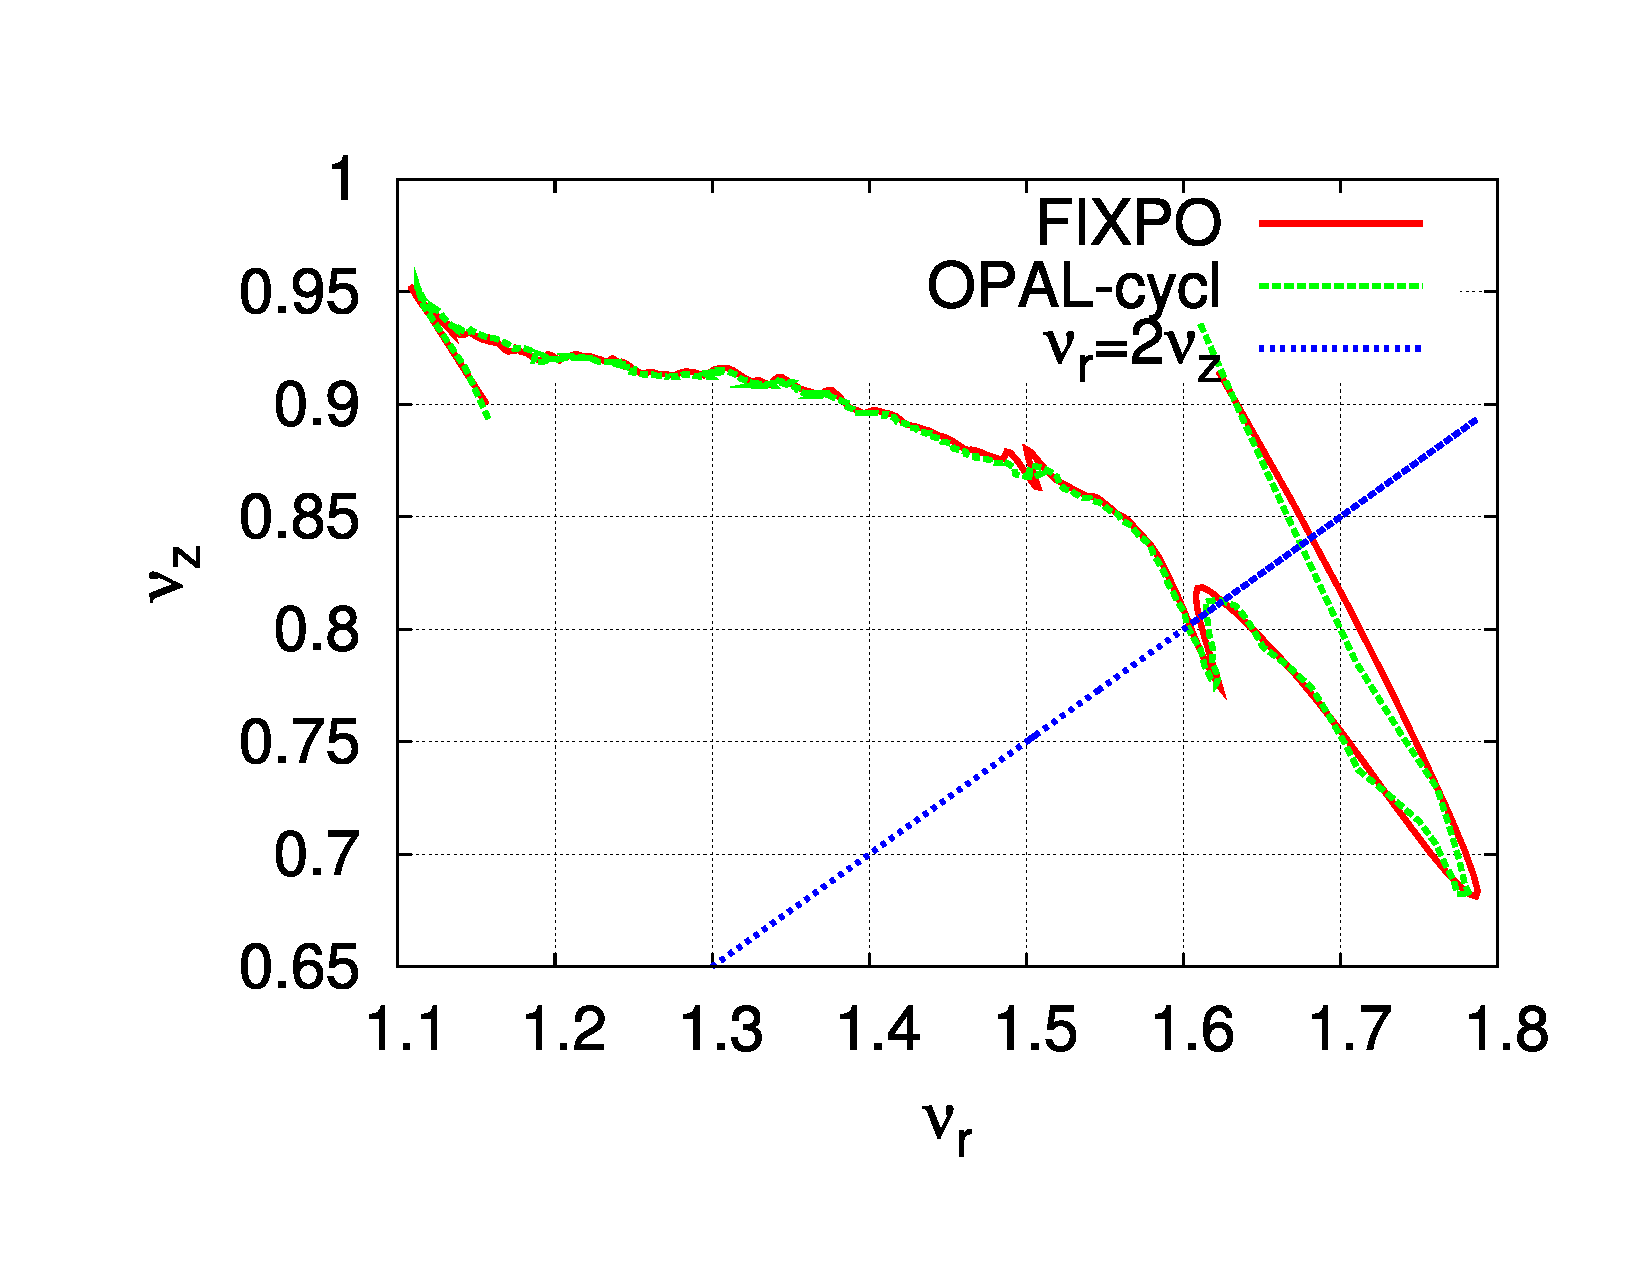
\includegraphics[width=\linewidth]{nurnuz_Ring} \\
      Tune calculation result is agree with FIXPO code very well!
    \end{column}
  \end{columns}
 % \end{block}
\end{frame}


\frame{
  \frametitle{PSI 590 MeV Ring - last 8 truns} 
 \framesubtitle{\alert{Compare with measured profiles}}


%  \begin{block}{Start-to-end RMS sizes comparison of a 3MeV beam}  
    \includegraphics[width=0.9\linewidth]{rre4v0120all}
   
 % \end{block}
}

\frame{
  \frametitle{Neighboring Bunch Effects- Multi Bunch Model}
  \begin{block}{}
    In our model, the injection-to-extraction simulation is divided into two stages,  
    \begin{itemize}
    \item First stage, big $\Delta R$  \alert{$\Rightarrow$}  single bunch tracking
    \item Second stage, small $\Delta R$ \alert{$\Rightarrow$}  multiple bunches tracking
    \item Full 3D
    \item Energy bins \& re-binning 
    \end{itemize} 
  \end{block}  
   \includegraphics[width=8cm]{SM-MultiBunch.pdf}
}


\frame{
  \frametitle{PSI 590MeV Ring}
  \framesubtitle{\alert{Single bunch}  and \alert{multiple bunches} at turn 80 and 130}
  
 \includegraphics[angle=90,width=0.95\linewidth]{C9B7BSB-2D-1mA-80.pdf}\\
 \includegraphics[angle=0,width=0.95\linewidth]{C9B7BSB-2D-1mA-130.pdf}

{\small Phys. Rev. ST Accel. Beams Volume 13 Issue 6 064201 (2010)}
}


%\begin{frame}{PSI 590MeV Ring}{\opalcycl Multiple bunches simulation of the Ring Cyclotron}
%\includemovie[
%poster,
%text=(Ring Cyclotron),
%mouse,
%repeat
%]{
%.8\linewidth
%}{
%.6\linewidth
%}{Movies/Ring9B3mA.mpeg}
%\end{frame}






\begin{frame}{Particle Matter Interaction}{}
%  \begin{block}{}  
 \begin{itemize}
 \item Energy loss $-dE/dx$ (Bethe-Bloch)
 \item Coulomb scattering is treated as two independent events: the multiple Coulomb scattering and the large angle Rutherford scattering
 \end{itemize}

A 72 MeV cold Gaussian beam with $\sigma_x=\sigma_y=5$ mm passing a copper slit with the half aperture of $3$ mm from 0.01 m to 0.1 m. 

The deflected particles contribute to the energy spectrum and angle deviation after a collimator. 

These particles may be lost downstream.
\end{frame}

\begin{frame}{Particle Matter Interaction cont.}{}
\begin{figure}[htb]
   \centering
  \includegraphics[width=0.9\linewidth]{trace3}
\end{figure}
 %\end{block}
\end{frame}


\begin{frame}{Particle Matter Interaction cont.}{}
 
\begin{figure}[htb]
   \centering
  \includegraphics[width=0.9\linewidth]{spectandscatter}
 \end{figure}

\end{frame}

\begin{frame}{Secondary Emission and Field Emission}{}
 


\end{frame}



\section{Conclusion and Outlook}

%\begin{frame}{Conclusion and Outlook}{Kurzweil - from  The Age of Spiritual Machines}
%\setbeamercovered{invisible}
%
%%\begin{block}{}
%\begin{center}
%%figures/PPTExponentialGrowthof_Computing
%\includegraphics<1>[width=0.85\linewidth]{Kur-Cycl1}
%\includegraphics<2>[width=0.85\linewidth]{Kur-Cycl2}
%\end{center}
%%\end{block}
%\end{frame}


\begin{frame}{Conclusion and  Outlook}{}

\begin{itemize}
\item Some of the ongoing efforts towards precise S2E beam dynamics simulations where sketched and parts of our results presented.
\item Using the HPC technology will enable us to speedup computations while increasing the accuracy of the used models: good statistics w.r.t losses $\rightarrow $ precise beam dynamics simulations!
\item HPC technology is not enough: more accurate modeling, using the state-of-the-art numerical methods (Master \& Ph.D projects) and adequate software technology is mandatory! 

\end{itemize}
\alert{The \opal framework tries to combine these essential factors which will enables us to enter into
new regimes of accelerator modeling and controls.}


\end{frame}

%\frame{
%\frametitle{Outlook: Dark Current \& Multipacting Simulations}
%\includemovie[
%poster,
%text=(Dark Current),
%mouse,
%repeat
%]{
%.8\linewidth
%}{
%.6\linewidth
%}{Movies/dc-1.avi}

%
%}





%\addtocounter{framenumber}{-12}
\setbeamertemplate{footline}[default]

	\begin{frame}
	  	\frametitle{Backup}
		\begin{center}
			\color{blue}{\LARGE{Backup}}
		\end{center}
	\end{frame}



%
% B A C K U P -- S L I D E S
%

\begin{frame}[fragile]
\begin{block}{}
\begin{verbatim}

GME:GEOMETRY, LENGTH=1, S=0.0, A=0.00085, B=0.00085;

Fs1:FIELDSOLVER, FSTYPE=MG, MX=32, MY=32, MT=64, 
        PARFFTX=false, PARFFTY=false, PARFFTT=true,
        BCFFTX=dirichlet, BCFFTY=dirichlet, BCFFTT=open, 
        GEOMETRY="GME", ITSOLVER="CG", INTERPL="linear",
        TOL=1e-6, MAXITERS=100, PRECMODE="reuse";

Fs2:FIELDSOLVER, FSTYPE=FFT, MX=32, MY=32, MT=64, 
        PARFFTX=false, PARFFTY=false, PARFFTT=true,
        BCFFTX=open, BCFFTY=open, BCFFTT=open,
        BOXINCR=1.0, GREENSF=INTEGRATED;

beam1: BEAM, PARTICLE=ELECTRON, PC=P0, NPART=1e5, 
	      BFREQ=1498.953425154e6, BCURRENT=0.299598, CHARGE=-1;

SELECT, LINE=FIND1;
\end{verbatim}
\end{block}
\end{frame}

\begin{frame}[fragile]
%\frametitle{\opal and its Flavours} 
%\framesubtitle{Sketch of an inputfile - \opalt cont.}
\begin{block}{}
\begin{verbatim}
TRACK,LINE=FIND1, BEAM=beam1, MAXSTEPS=10000, DT=1.0e-12;
 RUN, METHOD = "PARALLEL-T", BEAM=beam1, 
 FIELDSOLVER=Fs2, DISTRIBUTIONS={Dist1,Dist2};
endtrack;

f1: Filter, TYPE="FixedFFTLowPass", NFREQ=9;
f2: Filter, TYPE="Savitzky-Golay", NLEFT=64, 
	NRIGHT=64,POLYORDER=1;
CSRWAKE: Wake, TYPE="1D-CSR", FILTERS={f2, f1};

F10BC_MB01: RBend, L=0.282000, K0=0.1585,  
	FMAPFN="F10BC-MB01.T7", ELEMEDGE=29.964, 
	ALPHA=3.035,  DESIGNENERGY=247.6, WAKEF=CSRWAKE;
\end{verbatim}
\end{block}
\end{frame}


\begin{frame}[fragile]
%\frametitle{\opal and its Flavours} 
%\framesubtitle{Sketch of an inputfile - \opalt cont.}
\begin{block}{}
\begin{verbatim}
KX1I_PHYS: SurfacePhysics, TYPE="Collimator",MATERIAL="Cu";

KX0I: ECollimator, L=0.09, ELEMEDGE=0.01, 
	XSIZE=0.003, YSIZE=0.003, 
	APERTURE={0.003,0.003},SURFACEPHYSICS='KX1I_PHYS';

DR1:DRIFT, L=0.09, ELEMEDGE=0.01,
	APERTURE={0.003,0.003}, SURFACEPHYSICS='KX1I_PHYS';

QXA1:QUADRUPOLE,L=0.19,ELEMEDGE=0.11,K1=1.0,
	APERTURE={0.003,0.003}, SURFACEPHYSICS='KX1I_PHYS';

MXP00: Monitor, L=0.002, ELEMEDGE=0.1, OUTFN="MXP00.h5";

IW2Line: Line=(MXP00,KX0I);
\end{verbatim}
\end{block}
\end{frame}


\frame{
   \frametitle{870 keV Injection Line}
  \framesubtitle{\alert {Simulation} and \alert{measurement} DC beam 870 keV}
 
  \begin{columns}
    \begin{column}{6.0cm}
     \begin{block}{}
{\bf Estimate $\mathcal{D}_{start}$ and $\nu_e$ by $min(F)$:}
\[
F =\sum_{n=1}^{\#monitors}{(\rms{\mathcal{X}}_{mea}(s_n)-\rms{\mathcal{X}}_{sim}(s_n))^2} .
\]
\end{block}
    \end{column}
    \begin{column}{5.0cm}  
     \begin{overprint}
      \includegraphics<1>[keepaspectratio=true,width= 1.0\linewidth,angle=90]{beamline_without_accelerator_870keV} 
      \includegraphics<2>[keepaspectratio=true,width= 0.99\linewidth,angle=0]{MWP30}
      \end{overprint}
    \end{column}
  \end{columns}

}

\frame{
   \frametitle{870 keV Injection Line}
  \framesubtitle{\alert {Simulation} and \alert{measurement} DC beam 870 keV}
 
{\bf Find $\mathcal{D}_{start}$ and $\nu_e$ by $min(F)$:} $F =\sum_{n=1}^{\#monitors}{(\rms{\mathcal{X}}_{mea}(s_n)-\rms{\mathcal{X}}_{sim}(s_n))^2} .$
 %beamline_without_accelerator_870keV
    \begin{center}
     %\begin{overprint}
      \includegraphics<1>[keepaspectratio=true,width= 0.50\linewidth,angle=90]{870line} 
      \includegraphics<2>[keepaspectratio=true,width= 0.45\linewidth,angle=0]{MWP30}
      %\end{overprint}
 \end{center}
}

\frame{
  \frametitle{Comparison of beam profile monitors in the PSI-IW2 Line}
      \includegraphics[width=0.9\linewidth]{MNP1920.pdf}
}

\frame{
  \frametitle{Comparison of beam losses on the slits with measurements}
      \includegraphics[width=1.0\linewidth]{FX16.pdf}
}

\begin{frame} 
  \frametitle{Parallel Scalability: \small{Test on Cray XT3 at CSCS, Switzerland}}
  \begin{columns}
    \begin{column}{4.cm}
      \scriptsize
      \begin{block}{Setup}
        \begin{itemize}
        \item  \alert{$10^6$} particles, 
        \item 3D FFT on a  \alert{$64^3$} grid,
	\item \alert{2D} domain decomposition
	\item Track  \alert{200} time steps
        \item Gaussian distribution
	\item Dump data into \alert{single} H5Part file every 10 steps
        \end{itemize}
      \end{block}
      
      \begin{block}{Observations}
        \begin{itemize}
        \item The code scales well
	\item Good load-balancing
	\item I/O time is increasing 
        \end{itemize}
      \end{block}
    \end{column}
    \begin{column}{6.5cm}
%    \begin{block}{}    
      \includegraphics[width=0.95\linewidth]{Timing64mesh}
      \center Time to solution is reduced approximately by a factor of \alert{60}, (256P Vs 1P).
   % \end{block}  
    \end{column}
  \end{columns}
\end{frame}



\begin{frame}
		\frametitle{\oursolver\ Parallel Efficiency}
		
		\begin{columns}
		\begin{column}{6.5cm}
            \centering
		        \includegraphics[width=0.99\textwidth]{eff_1024_lin-crop.pdf}
        \end{column}
        \begin{column}{4.5cm}
            \begin{itemize} 
                \item obtained for a tube embedded in a $1024\times1024\times1024$ grid
                \item construction phase is performing the worst with an efficiency of 73\%
                \item influence of problem size on the low performance of the aggregation in ML
            \end{itemize}
        \end{column}
        \end{columns}

	\end{frame}



\end{document}





